% fig_ibr_element_breakdown.tex
% TR-27: Element firing breakdown for Part B internal IBR scenarios (N=9)
%
% Grouped bar chart: each scenario shows which elements fired.
% TDCS fires universally; 87L fires for k_ibr >= 0.12; 87LN0 for earthed SLG.
%
% Data from run_system_integration_v2.py Part B (internal scenarios only):
%   Scen 1: 3PH k=0.08      87L=0  87LN=0  87LN0=0  TDCS=1
%   Scen 2: 3PH k=0.15      87L=1  87LN=0  87LN0=0  TDCS=1
%   Scen 3: 3PH f=48.5Hz    87L=0  87LN=0  87LN0=0  TDCS=1
%   Scen 4: 3PH I_h3=0.08   87L=0  87LN=0  87LN0=0  TDCS=1
%   Scen 5: 3PH k=0.06 hi   87L=0  87LN=0  87LN0=0  TDCS=1
%   Scen 6: SLG solid        87L=0  87LN=0  87LN0=1  TDCS=1
%   Scen 7: SLG R-earth      87L=0  87LN=0  87LN0=1  TDCS=1
%   Scen 8: SLG unearthed    87L=0  87LN=0  87LN0=0  TDCS=1
%   Scen 9: SLG worst        87L=0  87LN=0  87LN0=0  TDCS=1
%
% Summary: 87L=1/9, 87LN=0/9, 87LN0=2/9, TDCS=9/9
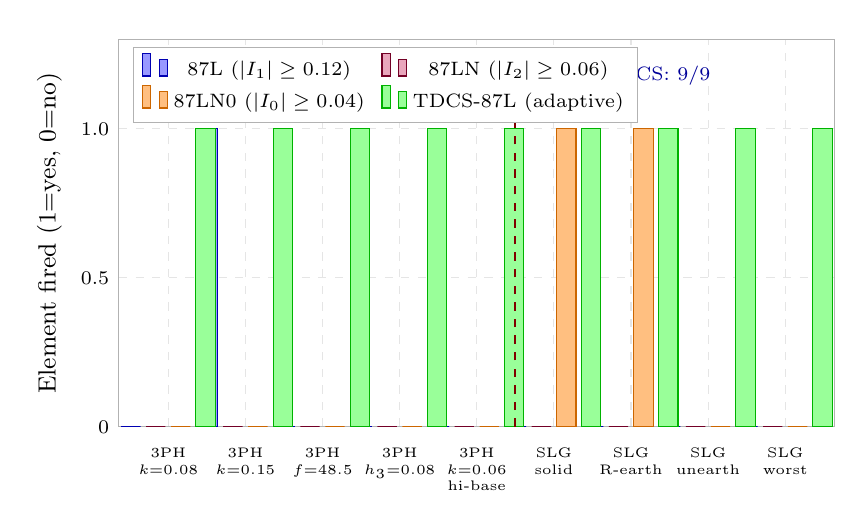
\begin{tikzpicture}
\begin{axis}[
  name        = elemax,
  ybar,
  bar width   = 7pt,
  width       = 0.88\textwidth,
  height      = 6.5cm,
  ylabel      = {Element fired (1=yes, 0=no)},
  ylabel style= {font=\small},
  ymin=0, ymax=1.30,
  ytick       = {0, 0.5, 1.0},
  yticklabels = {0, 0.5, 1.0},
  yticklabel style={font=\scriptsize},
  xtick       = {1,2,3,4,5,6,7,8,9},
  xticklabels = {3PH\\$k{=}0.08$,
                 3PH\\$k{=}0.15$,
                 3PH\\$f{=}48.5$,
                 3PH\\$h_3{=}0.08$,
                 3PH\\$k{=}0.06$\\hi-base,
                 SLG\\solid,
                 SLG\\R-earth,
                 SLG\\unearth,
                 SLG\\worst},
  xticklabel style={font=\tiny, align=center},
  enlarge x limits=0.08,
  legend style={at={(0.02,0.98)}, anchor=north west,
                font=\scriptsize, draw=gray!60,
                /tikz/every even column/.append style={column sep=4pt}},
  legend columns=2,
  grid       = major,
  grid style = {gray!20, dashed},
  tick style = {draw=none},
  axis line style={gray!60},
]

% 87L (blue)
\addplot[fill=blue!40, draw=blue!70!black]
  coordinates { (1,0)(2,1)(3,0)(4,0)(5,0)(6,0)(7,0)(8,0)(9,0) };
\addlegendentry{87L ($|I_1|\geq 0.12$)}

% 87LN (purple)
\addplot[fill=purple!35, draw=purple!60!black]
  coordinates { (1,0)(2,0)(3,0)(4,0)(5,0)(6,0)(7,0)(8,0)(9,0) };
\addlegendentry{87LN ($|I_2|\geq 0.06$)}

% 87LN0 (orange)
\addplot[fill=orange!50, draw=orange!80!black]
  coordinates { (1,0)(2,0)(3,0)(4,0)(5,0)(6,1)(7,1)(8,0)(9,0) };
\addlegendentry{87LN0 ($|I_0|\geq 0.04$)}

% TDCS (green)
\addplot[fill=green!40, draw=green!70!black]
  coordinates { (1,1)(2,1)(3,1)(4,1)(5,1)(6,1)(7,1)(8,1)(9,1) };
\addlegendentry{TDCS-87L (adaptive)}

% Fault type divider at x=5.5
\draw[red!50!black, thick, dashed]
  (axis cs:5.5, 0) -- (axis cs:5.5, 1.20);
\node[font=\tiny, red!60!black, align=center]
  at (axis cs:5.5, 1.25) {3PH | SLG};

% Summary annotation
\node[font=\scriptsize, blue!60!black, align=left]
  at (axis cs:5.0, 1.18)
  {87L: 1/9\quad 87LN: 0/9\quad 87LN0: 2/9\quad TDCS: 9/9};

\end{axis}
\end{tikzpicture}
